\section{Etudes préalables}

Avant de commencer à parler de tout l’aspect technique et conception nous allons resituer notre projet en définissant ses objectifs, son plan de route et ses inspirations.

\subsection{Présentation du projet}

Ce projet a été mis en place de notre propre initiative et nous avons donc défini les objectifs à atteindre ainsi que les fonctionnalités de nous-même, avec l'aide du tuteur de projet.

L’idée originelle que nous avions proposée était inspirée de la carte du Maraudeur de l’univers Harry Potter visible sur la figure \ref{marauder}. Cette carte permet grâce à la magie de suivre en temps réel toutes les personnes présentes à Poudlard, l’école de sorciers, puisque leurs pas apparaissent dessus avec leur nom. Cet objet, bien que magique, nous semblait aujourd’hui pouvoir être réalisé grâce aux avancées liées au domaine des objets connectés. 

\begin{figure}[H]
    \centering
    \includegraphics{./img/marauder.jpg}
    \caption{Morceau de la carte du Maraudeur tirée du film}
    \label{marauder}
\end{figure}

Nous avons donc décidé de proposer une manière simple pour tout le monde de pouvoir s'orienter et retrouver des personnes dans les locaux de l'ISIMA au travers d’une application. Cette solution devra donc récolter l’ensemble des données sur les usagers de l’ISIMA et les reporter sur une carte qui sera bien sûr électronique. Nous voulons ainsi que chacun puisse sortir notre carte de sa poche pour retrouver un ami ou un collègue instantanément.

De manière générale, nous devons être capable de visualiser une carte de l'ISIMA, mais également de pouvoir trouver facilement une personne, un bureau ou une salle de cours. De plus, il serait intéressant de pouvoir localiser n'importe quelle autre personne sur la carte en temps réel. Cette visualisation doit s'actualiser assez rapidement pour que la localisation de personnes soit la plus précise possible pour les utilisateurs.

Une fois cette solution éprouvée avec les bâtiments de l'ISIMA, nous pouvons penser l'étendre à n'importe quel autre bâtiment dont nous pouvons avoir les plans. L’intérêt ici étant de développer une preuve de fonctionnement du suivi de personnes dans un bâtiment qui plus est considéré comme étant très surchargé de signaux. Comme nous l’évoquions plus tôt ceci pourrait trouver différentes utilisations dans différents contextes comme par exemple le fonctionnement d’un hôpital, la surveillance d’une prison, l’évacuation d’un bâtiment. Avec l’avènement de l’open data, il y a aussi de nombreuses questions éthiques à résoudre vis-à-vis des informations récoltées et diffusées.


\subsection{Analyse de l'existant}

Nous ne nous attarderons pas dans cette partie sur la carte magique imaginée par J. K. Rowling mais nous allons plutôt voir les différentes applications existant autour de la localisation d’usagers.

Le premier exemple est celui des réseaux sociaux. En effet, avec leur avènement est arrivé aussi un moyen pour des grands groupes de récolter une masse importante d’information sur leurs utilisateurs : ce que l’on appelle le Big Data. Dans cette masse de données, il y a bien évidemment des données de géolocalisation. Celles-ci sont de plusieurs types : soit données, soit mesurées.

Les premières, dites données, sont les informations que l’utilisateur va donner de lui-même aux réseaux sociaux comme par exemple poster une photo d’une après-midi entre amis en spécifiant le lieu de la prise de vue. Cette information peut être légitimement utilisée puisque donnée par l’utilisateur mais cela ne représente pas une source fiable ni même précise. Même si cette information n’est pas fiable, les réseaux sociaux ont trouvé depuis 2014 une toute nouvelle utilisation à ce type d’information : l’aide aux personnes en danger. En effet, Facebook a développé un service nommé Safety Check qui repère les personnes présentes à proximité d’une zone de danger que ce soit une catastrophe naturelle ou bien encore une action terroriste et leur propose de se signaler en sécurité auprès de leurs proches. Le Safety Check visible à la figure \ref{safety-check} est un bon exemple de localisation de personnes mais demande à ce que les personnes recherchées effectuent une action.

\begin{figure}[H]
    \centering
    \includegraphics{./img/safety-check.png}
    \caption{Service Safety Check de Facebook}
    \label{safety-check}
\end{figure}

Le second type dit données mesurées représente toutes les informations que les réseaux sociaux récupèrent sur les appareils des utilisateurs. Cette récupération est rendue possible tout d’abord par l’existence de ces données. En effet depuis quelques années avec l’arrivée des smartphones et des objets connectés, la majeure partie des appareils électroniques possèdent des fonctionnalités de géolocalisation. Il est alors facile pour une application d’accéder à la position de son utilisateur. En général, l’appareil en question est un smartphone et se trouve très souvent au même endroit que son propriétaire, voire sur lui-même. On peut clairement constater la récupération de ces informations lorsque la localisation d’un utilisateur est associée directement au message qu’il poste ou bien encore sur les historiques. En effet, Google propose à ses utilisateurs d’accéder à tous l’historique de leurs déplacements comme on peut le voir sur la figure \ref{google-maps}. Google récupère en permanence la position de utilisateurs afin de pouvoir fournir à la communauté des statistiques sur l’affluence de certains lieux, de demander des informations et photos sur les lieux en cours de visite ou bien proposer des services à proximité. Google arrive ici à localiser avec précision dans quel établissement une personne se trouve mais ne partage pas les données individuelles au reste de la communauté.

\begin{figure}[H]
    \centering
    \includegraphics{./img/google-maps.png}
    \caption{Suivi des déplacement sur Google Maps}
    \label{google-maps}
\end{figure}

KHEOLY RENNES

APPLICATION ANDROID

\subsection{Spécifications du projet}

Etant donné que peu de solutions sont disponibles sur le marché, nous avons choisi de partir de zéro et créer notre solution. Cela nous permet également d'avoir un contrôle total sur les données, du projet, les diverses implémentations de fonctionnalités ainsi que la manière dont nous souhaitons utiliser notre solution.

La solution la plus évidente en termes de support de visualisation pour les utilisateurs et de leur proposer une application qu'ils pourront installer sur leur smartphone, pc, montre connectée ou encore tablette.
Afin de rendre cette application dynamique et de proposer un suivi de position d'utilisateurs en temps réel, il est convenu d'utiliser un Service Web. Ce service permettra également de stocker des informations utiles aux utilisateurs, ce qui permettra également d'alléger le volume de données stockées sur leurs terminaux.

\subsubsection{Architecture}

L'architecture choisie pour organiser notre solution est la suivante.

\begin{figure}[H]
    \centering
    \includegraphics[height=10cm]{../infrastructure.png}
    \caption{Architecture}
    \label{architecture}
\end{figure}

Nous pouvons observer dans la figure~\ref{architecture} que celle-ci ressemble à une architecture client/serveur, ce qui est le but recherché.

\subsubsection{Partie serveur}
La partie centrale est celle du Web Service. Le serveur doit etre capable de répondre aux différentes connexions et requêtes des utilisateurs (se connectant sur l'application Android ou tout autre...). Le serveur sera un Service Web de type \textbf{REST} disposant pour fonctionnalités minimales :
\begin{itemize}
    \item de s'authentifier ;
    \item d'obtenir les positions d'autres personnes connectées sur l'application ;
    \item obtenir la liste des personnes connectées ;
    \item envoyer la position actuelle de l'utilisateur connecté ;
    \item se déconnecter.
\end{itemize}

Ces fonctionnalités seront essentielles pour le fonctionnement de base de l'ensemble de la solution. Par la suite, des fonctionnalités supplémentaires pourront être ajoutées dans l'application, par exemple :
\begin{itemize}
    \item historique des positions ;
    \item calcul d'itinéraire entre 2 positions dans le bâtiment ;
    \item partage de position (par sms, mail, ...).
\end{itemize}

Pour stocker les diverses informations utilisateur (login, position), nous avons convenu d'utiliser une base de données qui s'interfacera directement avec le Service Web.

\subsubsection{Partie Android}
Une seconde partie comporte une application Android (qui pourrait être déclinée pour iOS et Windows Phone). Cette application permettra :
\begin{itemize}
    \item de s'inscrire
    \item de se connecter
    \item envoyer sa position gps au service web
    \item recevoir les positions gps d'autres utilisateurs connectés
    \item visualiser en temps réel sur une carte les positions
\end{itemize}

L'application pourra évoluer et proposer :
\begin{itemize}
    \item la carte en version 3D
    \item la carte en version VR
    \item l'ajout d'informations sur la carte (lieu / point de rdv)
\end{itemize}

Le choix d'une application Android se justifie par :
\begin{itemize}
    \item la communauté Android est active
    \item la quantité de terminaux
    \item l'un de nous a des connaissances en Android
\end{itemize}
La mise à jour des positions est soit faite par l'application qui effectue une requête sur le serveur, soit c'est le serveur qui renvoie les positions des utilisateurs ayant bougé d'un delta suffisant qui permet sa mise à jour chez les utilisateurs. Les frameworks 3.X+ seront supportés pour fonctionner sur un maximum de terminaux.


\subsubsection{Intégration continue}
Un des objectifs de ce projet est de mettre en place une intégration continue et un déploiement automatique. Pour ce faire il est nécessaire d'avoir deux serveurs :
\begin{itemize}
    \item un serveur d'application
    \item un serveur d'intégration
\end{itemize}

Le premier sera certainement un CaaS Amazon pour NodeJS. Le serveur d'intégration sera un serveur Travis CI puisqu'il gère à la fois le NodeJS et l'Android (nouvelle fonctionnalité). Cela permettra contrairement à un serveur Jenkins de déployer facilement sans avoir à gérer un serveur mais juste en utilisant un service.

\subsection{Organisation du travail}

L'organisation temporelle théorique du travail est décrite dans le diagramme de Gantt ci-dessous.

\begin{landscape}
    \begin{figure}[h]
        \centering
        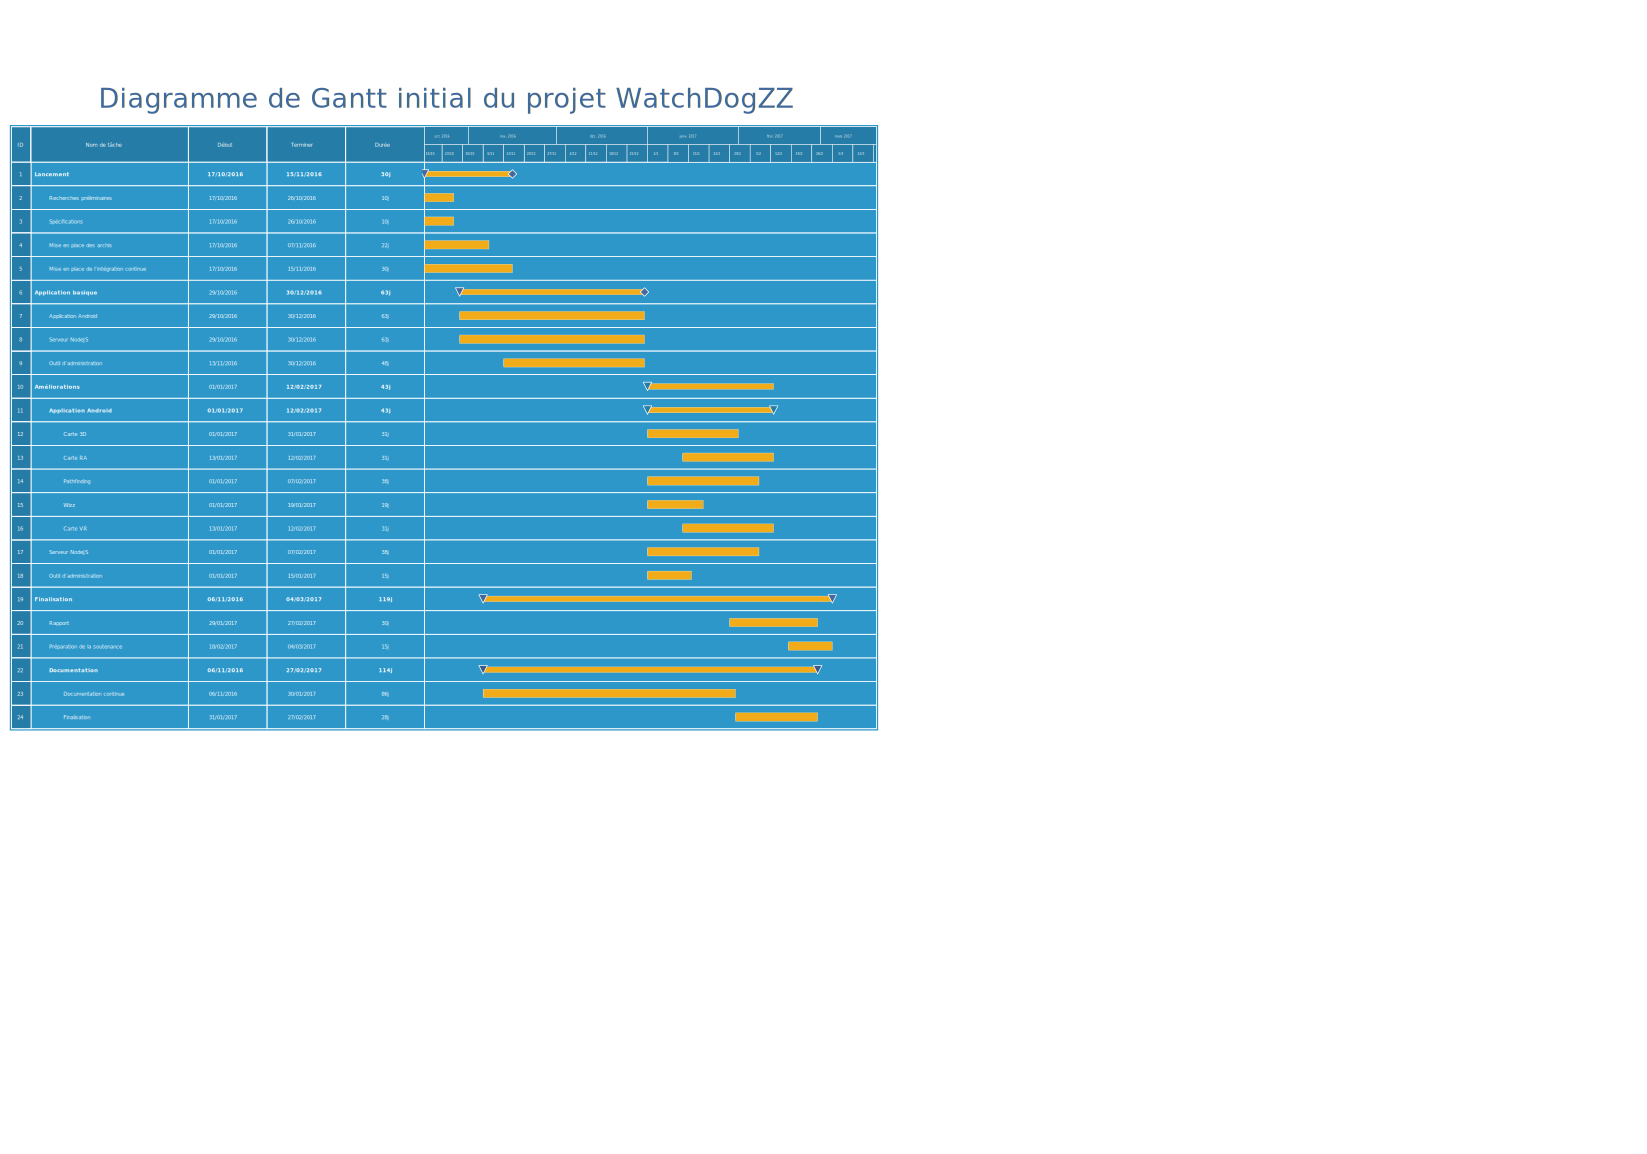
\includegraphics[height=\textwidth]{../gantt_initial.png}
        \caption{Diagramme de Gantt théorique}
    \end{figure}
\end{landscape}

suite...
